% Sandia National Laboratories is a multimission laboratory managed and
% operated by National Technology & Engineering Solutions of Sandia, LLC, a
% wholly owned subsidiary of Honeywell International Inc., for the U.S.
% Department of Energy’s National Nuclear Security Administration under
% contract DE-NA0003525.

% Copyright 2002-2019 National Technology & Engineering Solutions of Sandia,
% LLC (NTESS).


\begin{Device}\label{P_DEVICE}

%\symbol
%{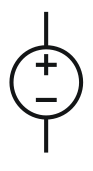
\includegraphics{ivsSymbol}}

\device
\begin{alltt}
V<name> <(+) node> <(-) node> port=port number  [Z0 = value]
+ [[DC] <value> ] [AC [magnitude value [phase value] ] ]  
+ [transient specification]
\end{alltt}

\examples
\begin{alltt}
P1 1 0 port = 1
P2 12 0  port=1  z0=100
P1 1 0 port=2   sin 0  1 1e5
P2 2 0 port=2 z0=100 AC 1
\end{alltt}


\parameters

\begin{Parameters}

\param{port}

The port number. Numbered sequentially beginning with 1

\param{Z0} 

System impedance. Currently, it only supports a real-valued impedance.

\param{transient specification}

There are six predefined time-varying functions for sources:

\begin{description}
\item[\tt PULSE <parameters>] Pulse waveform
\item[\tt SIN <parameters>] Sinusoidal waveform
\item[\tt EXP <parameters>] Exponential waveform
\item[\tt PAT <parameters>] Pattern waveform
\item[\tt PWL <parameters>] Piecewise linear waveform
\item[\tt SFFM <parameters>] Frequency-modulated waveform
\end{description}

\end{Parameters}

\comments

The port device identifies the ports used in .LIN analysis. Each
port requires a unique port number. For example, if the netlist has
N port devices, it must contain the sequential set of port
numbers, from 1 to N. Each port has an associated impedance Z0. The
default is 50 ohms. 

The port device behaves as a voltage source in series with an impedance
for all other analyses, such as DC, AC and transient.

None, any, or all of the DC, AC, and transient values
can be specified. The AC phase value is in degrees. The port device
accepts the same transient specifications as the voltage (V) sources.

\end{Device}

